\documentclass[a4paper]{article}
\usepackage[utf8]{inputenc}
\usepackage[slovene]{babel}
\usepackage[T1]{fontenc}
\usepackage{fullpage}
\usepackage{amsmath}
\usepackage{amssymb}
\usepackage{amsthm}
\usepackage{enumerate}
\usepackage{listings}
\usepackage{verbatim}
\usepackage{float}
\usepackage{graphicx}
\usepackage{epstopdf}
\usepackage{url}
\begin{document}
\begin{titlepage}
	\centering

	{\scshape\LARGE Univerza v Ljubljani \\Fakulteta za Matematiko in Fiziko \par}
	\vspace{1cm}
	{\scshape\Large Programiranje 1\par}
	\vspace{1.5cm}
	{\huge\bfseries Analiza iger na plaformi Steam \par}
	\vspace{2cm}
	{\Large\itshape Matej Neumann\par}
	\vfill

% Bottom of the page
	{\large \par}
\end{titlepage}

\section{Uvod}

S to nalogo želim analizirati kolekcijo iger na platformi Steam.
Steam je bil izbran ker je trenutno najbolj popularen in priljubljen distributor video iger za PC,MAC, in Linux.
Le-ta tudi shranjuje podatke za več kot 100 milijonov uporabnikov in več kot 20,000 iger kar pomeni da je idealen kandidat za analizo velike količine podatkov.


\subsection{Metacritic}

Čeprav je veliko podatkov samoumevnih bi Metacritic mogoče potreboval nekaj pojasnila.
Metacritic ponuja možnost ocenjevanja za video igere, filme, televizijske oddaje in glasbe.
Ocena Metacritik-a je uravnotežena med ocenami profesionalnih kritikov in publicistov na lestvici od 1 do 100.
Le-ta je tudi ena izmed najbolj pogosto uporabljenih lestic za določanje kvalitete video iger.

\subsection{Opomin}

Proces pridobivanja podatkov ni zmogel pridobiti vseh zaželjenih podatkov.
Nekateri podatki niso zabeleženi, do drugih pa lahko dostopa le administrator računa.
Število lastnikov ni mogoče dobiti, ampak je bil približek pridobljen iz strani \url{https://steamspy.com/}, prav tako ni bilo mogoče razlikovati med negativnimi in pozitivnimi priporočili zato se na to gleda samo kot priporočila.

\section{Napovedi}
Ker sem s platformo Steam dobro seznanjen sem naredil par napovedi za katere se bom kasneje tudi prepričal.
\begin{enumerate}
  \item Brezplačne igre dobijo povprečno več priporočil kot plačljive in imajo  nižjo oceno na Metacritiku
  \item Med najbolj igranimi igri bodo " Dota 2 " in "$\text{ Counter Strike Global Offensive}$"
  \item Najbolj popularna žanra bo action
  \item Število povprečno število DLC-ov na igro se je v zadnjem letu drastično povečalo
  \item povezave med ceno igre in njeno oceno ne bo ali bo kvečjemu padala z oceno
\end{enumerate}

\newpage
\section{Rezultati}

\subsection{Brezplačne vs plačljive}
Kot pričakovano brezplačne igre res dobijo v povprečju več priporočil kot plačljive (Slika \ref{fig:freevspaid_rating}).
in na prvi pogled imajo tudi večjo oceno (Slika \ref{fig:Freevspaid_score}), kar pa se izkaže da ni res.
Šel sem namreč pogledati še povprečne ocene za vsak žanr posebi (Slika \ref{fig:score-by-genre})
in tu izvemo  da je žanra "Free To Play" četrte najslabše ocenjena, kar se ujema z pričakovanji . Zakaj potem še vedno v povprečju dosegajo brezplačne boljše ocene?
Problem je v tem da Steam nekaterim igra doda atribut "IsFree" kljub temu da je za igro treba plačati (igre namreč lahko vspadajo v nek paket "bundle" za katere je treba plačati kljub temo da piše da je igra sama nima cene) in ker je brezplačnih iger
ki imajo oceno na Metacritiku relativno malo lahko to hitro vpliva na povprečno oceno. Iz tega lahko sklepa da brezplačne igre v povprečju res dobijo več priporočil in imajo slabše ocene.
\begin{figure}[h]
    \centering
    \begin{minipage}{0.45\textwidth}
			\centering
			\caption{število priporočil pri primerjavi men brezplačnimi in plačljivimi \label{fig:freevspaid_rating}}
			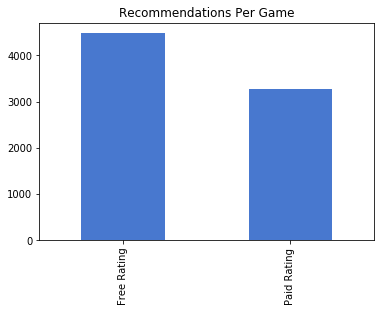
\includegraphics[width=1\textwidth,keepaspectratio]{graf_stevilo_ocen.png}
    \end{minipage}\hfill
    \begin{minipage}{0.45\textwidth}
			\centering
			\caption{število priporočil pri primerjavi men brezplačnimi in plačljivimi \label{fig:Freevspaid_score}}
			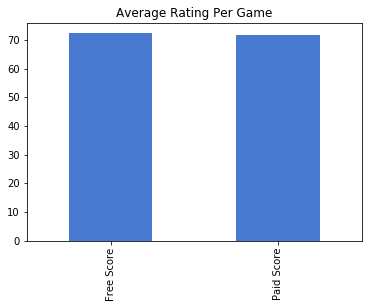
\includegraphics[width=1\textwidth,keepaspectratio]{graf_povprecna_ocena.png}
    \end{minipage}
\end{figure}
\begin{figure}[h]
    \centering
    \begin{minipage}{0.45\textwidth}
				\caption{povprečna ocena glede na žanr}
			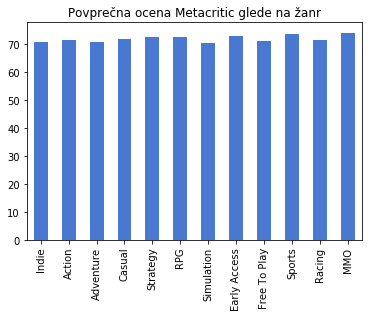
\includegraphics[width=1\textwidth,keepaspectratio]{zanr-meta-pov.png}

			\label{fig:score-by-genre}
    \end{minipage}\hfill
\end{figure}
\newpage
\subsection{Najbolj popularne igre }
Kot pričakovano so še vedno najbolj popularne iste igre kot pred leti.
Večina teh iger ima tudi  svojo E-sport ligo (Dota 2 , Counter Strike Global Offensive), kjer igralci ( ponavadi v ekipah) tekmujejo proti drugimi v živo in v finalih tudi za veliko količio denarja.
Veliko presenečenje je PLAYERUNKNOWNS BATTLEGROUNDS 	ki je lansko leto prišla od nikoder in je sedaj ena izmed najbolj gledanih in popularnih iger na Steamu.

\begin{figure}[h]
    \centering

			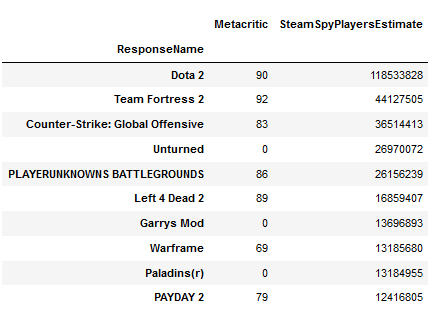
\includegraphics[width=0.45\textwidth,keepaspectratio]{Top10MostPlayed.png}
			\caption{Najbolj igrane igre}
			\label{fig:most-played}

\end{figure}

\subsection{Najbolj popularna žanra}
Najbolj popularna žanra ni bila action temveč MMO, kateri  sta potem sledili action in Free To Play.
Vendar Kljub temu je bila action ena izmed najslabše ocenjenih žanr medtem ko sta bili MMO in sport najbolje ocenjeni (Slika \ref{fig:score-by-genre})

\subsection{DLC}
DLC ali downloadable content je nekakšen dodatek osnovni igri ki jo ne more zamenjati temveč je kvečjemu lahko  nadgradi. Zazdelo se mi je da se  število le-teh vedno večje vendar zgleda da se je pred časom trend obrnil  (Slika \ref{fig:dlc_per_year})
Še bolj zanimiva je pa slika  (Slika \ref{fig:known_unknown}) ki prikazuje število izdanih iger na leto in omogoča primerjavo med tistimi ki imajo oceno na Metacritiku in tistimi ki jo nimajo. Kot lahko vidimo se je v letu 2013-2014 zgodil velik skok,
saj je takrat Steam omogočil Greenlight, kar je pomenilo da njegova trgovina ni bila več strogo nadzorovana amapak so sedaj tudi drugi manj znani izdajalci naložili svoje igre in če so le-te dobile dovolj glasov so potem šle v prodajo.
\begin{figure}[h]
    \centering
    \begin{minipage}{0.45\textwidth}
			\centering
			\caption{število DLC-ov glede na leto \label{fig:dlc_per_year}}
			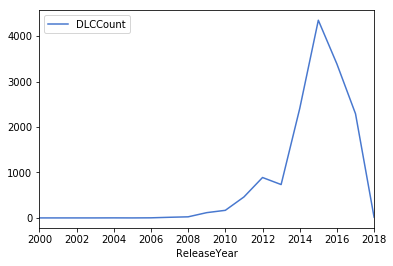
\includegraphics[width=1\textwidth,keepaspectratio]{graf_stevilo_dlc_leto.png}
    \end{minipage}\hfill
    \begin{minipage}{0.45\textwidth}
			\centering
			\caption{Število iger z znano oceno in neznano \label{fig:known_unknown}}
			\includegraphics[width=1\textwidth,keepaspectratio]{KnownvsUnknown.png}
    \end{minipage}
\end{figure}
\newpage
\subsection{Dodatne opazke}
Poleg ze dobljenih stvari me je zanimalo kakšna je bila povrečna ocena iger na leto. Ugotovil sem da kljub temo da povprečna ocena na leto pada se število dobrih iger vsako leto poveča.
(Slike \ref{fig:avg_r_year},\ref{fig:avg_n_year},\ref{fig:bad_n_year},\ref{fig:good_n_year}).
Še ena stvar ki se lahko opazi iz Slike \ref{fig:rec_meta} je da število priporočil res narašča z oceno, kar je pričakovano saj boljše igre igra več ljudi kar pomeni da bodo dobile več ocen.

\begin{figure}[h]
    \centering
    \begin{minipage}{0.45\textwidth}
			\centering
			\caption{Povprečna ocena na leto \label{fig:avg_r_year}}
			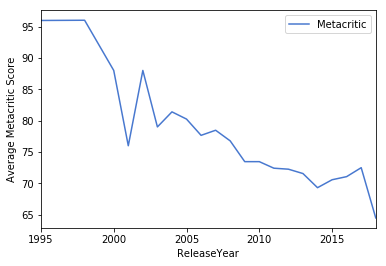
\includegraphics[width=1\textwidth,keepaspectratio]{fgraf_povprecna_ocena_leto.png}
    \end{minipage}\hfill
    \begin{minipage}{0.45\textwidth}
			\centering
			\caption{Število povprečnih iger \label{fig:avg_n_year}}
			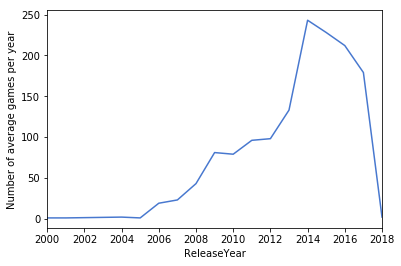
\includegraphics[width=1\textwidth,keepaspectratio]{graf_PovprecneIgre_leto.png}
    \end{minipage}
\end{figure}
\begin{figure}[h]
    \centering
    \begin{minipage}{0.45\textwidth}
				\caption{Število slabih iger}
			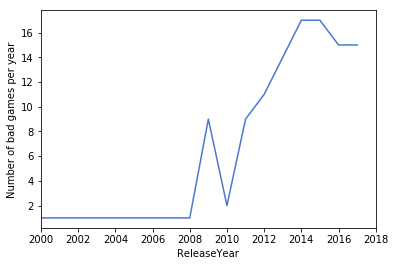
\includegraphics[width=1\textwidth,keepaspectratio]{graf_SlabeIgre_leto.png}

			\label{fig:bad_n_year}
    \end{minipage}\hfill
		\begin{minipage}{0.45\textwidth}
			\centering
			\caption{Število dobrih iger \label{fig:good_n_year}}
			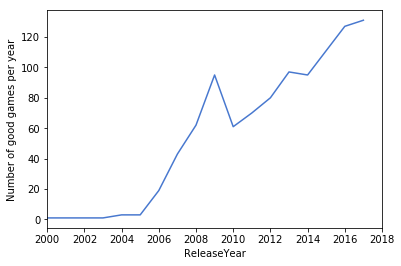
\includegraphics[width=1\textwidth,keepaspectratio]{graf_Dobre_leto.png}
    \end{minipage}
    \begin{minipage}{0.45\textwidth}
			\flushleft
				\caption{Število priporočil v odvisnosti od ocene}
			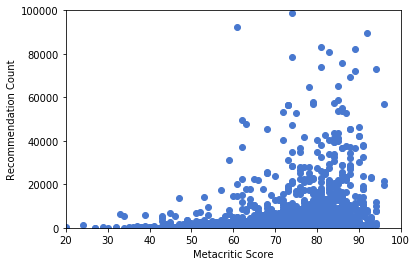
\includegraphics[width=1\textwidth,keepaspectratio]{graf_meta_rec.png}
			\label{fig:rec_meta}
    \end{minipage}\hfill
\end{figure}

\end{document}
